\subsection{CIT model diagnostics and robustness}
\label{sec:b-diagnostics}
% Owner: B. All diagnostics use the completed CIT run, not new experiments.
\paragraph{Null controls and ageing alternatives.}
\Cref{fig:b-null-age} visualizes the separation of the observed attachment
exponent from both null ensembles and the age-kernel AIC comparison.
P3b matches mean citation age because its age weights were fitted to these data;
that agreement is a property of the control, not independent evidence for ageing.
With only 20 realizations per null, an observed value above all nulls has empirical
one-sided probability $1/21$; this does not justify a precise tail estimate.
The ageing comparison is on identical risk sets and observations.

\begin{table}[t]
\centering\small
\begin{tabular}{@{}lrr@{}}
\toprule
Age kernel & Parameters & $\Delta$AIC\\
\midrule
Lognormal & 2 & 0.0\\
Exponential & 1 & 537.8\\
Power-law & 1 & 9,360.5\\
Uniform & 0 & 41,796.7\\
\bottomrule
\end{tabular}
\caption{CIT age-preference alternatives on common observed support. AIC selects
among the declared models, not among every possible ageing mechanism.}
\label{tab:b-age-models}
\end{table}

\begin{figure*}[t]
\centering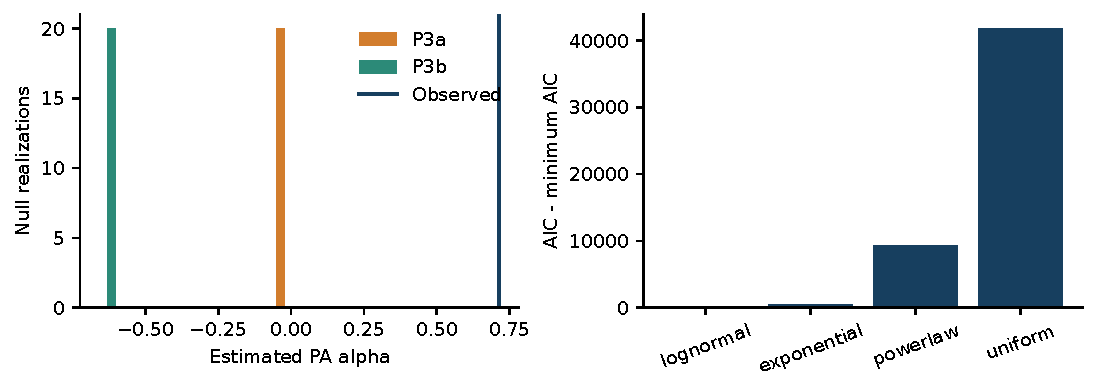
\includegraphics[width=.95\textwidth]{b_null_and_age_models.pdf}
\caption{CIT null-model attachment exponents and age-kernel AIC differences.
Uniform P3a and calibrated age-only P3b each have 20 independent realizations.}
\label{fig:b-null-age}
\end{figure*}

\paragraph{Fit quality does not establish predictability.}
The full-history sample is 500 of 1,019 papers with at least ten citations by age
15; the forecast sample is 500 of 1,220 eligible papers selected only by having
at least five citations in their first five years. Both samples are drawn with a
fixed seed. Median full-history RMSLE is 0.0736 and median scaled-collapse RMSE
0.0220 (90th percentile 0.0453); 10.2\% of full-history fits hit a parameter bound.
\Cref{fig:b-wsb-fits} is an in-sample diagnostic. Held-out scoring in
\cref{tab:b-forecast} and \cref{fig:b-wsb-validation} provides the separate
predictive test. In particular, a collapse obtained using parameters fitted to
the same curve is not independent evidence for universal citation dynamics.

\begin{figure*}[t]
\centering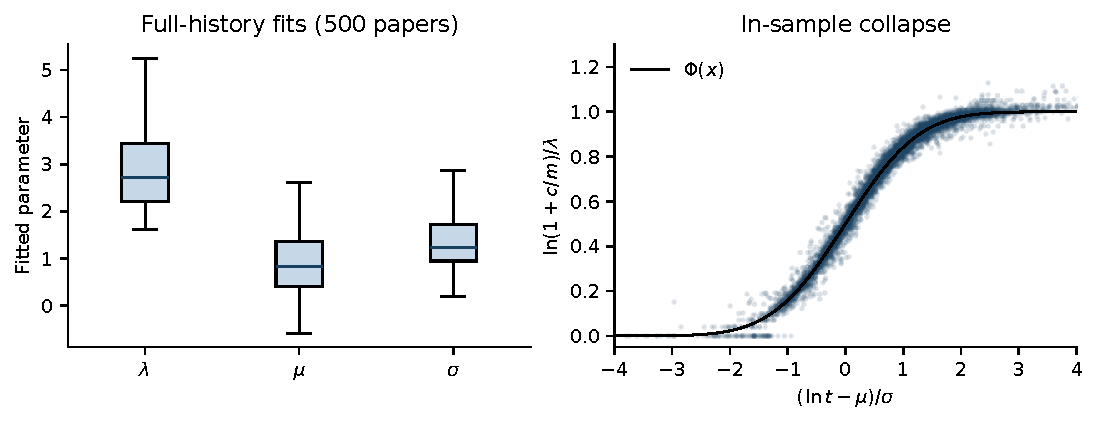
\includegraphics[width=.95\textwidth]{b_wsb_fit_diagnostics.pdf}
\caption{WSB full-history diagnostics: parameter distributions (boxes are
interquartile ranges, median lines, standard 1.5-IQR whiskers; outliers hidden)
and the scaled citation histories against $\Phi(x)$. Parameters are fitted to
ages 1--15, so the collapse is descriptive, not held-out validation.}
\label{fig:b-wsb-fits}
\end{figure*}

\begin{table}[t]
\centering\small
\setlength{\tabcolsep}{4pt}
\begin{tabular}{@{}llrr@{}}
\toprule
Target & Model & MAE & RMSLE\\
\midrule
15 yr & WSB & 15.144 & 0.601\\
 & Linear & 17.064 & 0.662\\
 & No-age PA & 27,588 & 4.601\\
\midrule
2020 & WSB & 28.016 & 0.778\\
 & Linear & 27.271 & 0.876\\
 & No-age PA & $2.79\!\times\!10^6$ & 7.000\\
\bottomrule
\end{tabular}
\caption{Matched forecasts on 500 selected papers using only years 1--5 for
training. The 2020 target is the observed, censored corpus endpoint.
The exponential no-age PA baseline over-extrapolates; beating it alone is a weak
test. The paired MAE intervals against linear both include zero.}
\label{tab:b-forecast}
\end{table}

\paragraph{Sensitivity of the conclusions.}
\Cref{tab:b-robustness} reports time splits, cutoff and corpus-selection checks.
The sign of degree preference and superlinear full-period growth persist, but
$a$ is substantially weaker in the late period. Degree offsets 0.5 and 2 give
$\alpha=0.604$ and 0.858, so the numerical exponent is convention-dependent.
Including 5,486 year ties gives $a=1.324$; ties remain excluded from the primary
DAG. Effective-diameter endpoint estimates remain 6 hops with 64, 128 or 256
sources. First-ten versus all-twenty null means of $\alpha$ are 0.00055/0.00059
(P3a) and $-0.65320$/$-0.65118$ (P3b).
Lognormal ageing is preferred in all target cohorts and both observation halves,
but the recent cohort's fitted tail extends beyond its observed follow-up.
These checks support qualitative stability without eliminating coverage bias,
right censoring or unobserved fitness.

\begin{table}[t]
\centering\small
\begin{tabular}{@{}lrr@{}}
\toprule
Variant & $\alpha$ & $a$\\
\midrule
1990--2020 (primary) & 0.714 & 1.343\\
1990--2004 & 0.684 & 1.455\\
2005--2020 & 0.721 & 1.065\\
Cutoff 2015 & 0.722 & 1.427\\
Core venue families & 0.731 & 1.410\\
Same-year edges included & -- & 1.324\\
\bottomrule
\end{tabular}
\caption{CIT robustness from the saved run. Core venue families contain 14,235
nodes and 47,009 primary edges; the year-tie variant is structural only.}
\label{tab:b-robustness}
\end{table}
